\section{Schematy funkcjonalne układu}

\subsection{Schemat blokowy analizatora}
Analizator stanów logicznych składa się z 3 głównych bloków:
\begin{enumerate}
    \item Układu wejściowego
Układ wejściowy analizatora zapewnia dostęp do 16 wejść cyfrowych,
2 szybkich wejść analogowych niskiej rozdzielczości 2 wolnych wejść
analogowych dużej rozdzielczości oraz 4 złącz masy. Szczegółowy opis 
interfejsu wejściowego analizatora przedstawiono poniżej.
\begin{figure}
    \centering
    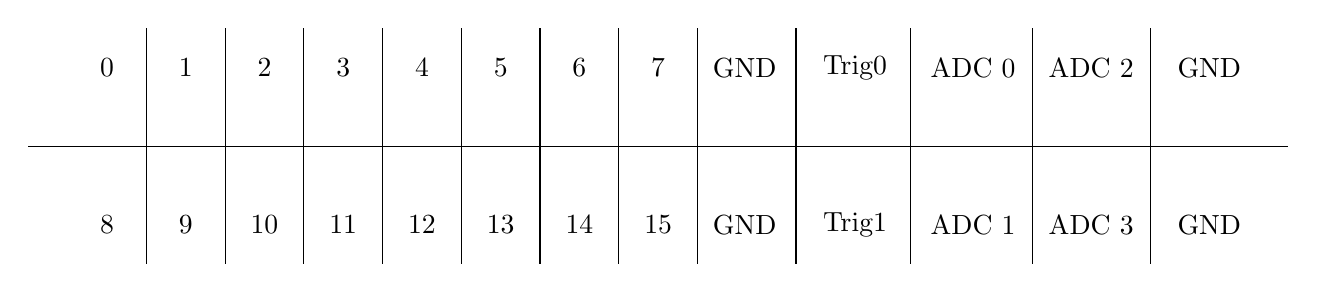
\begin{tikzpicture}
        \draw
            (-1, 0) -- (15, 0)

            (0, 1) node[]{0}
            (1, 1) node[]{1}
            (2, 1) node[]{2}
            (3, 1) node[]{3}
            (4, 1) node[]{4}
            (5, 1) node[]{5}
            (6, 1) node[]{6}
            (7, 1) node[]{7}

            (0, -1) node[]{8}
            (1, -1) node[]{9}
            (2, -1) node[]{10}
            (3, -1) node[]{11}
            (4, -1) node[]{12}
            (5, -1) node[]{13}
            (6, -1) node[]{14}
            (7, -1) node[]{15}

            (8.1, 1) node[]{GND}
            (8.1, -1) node[]{GND}

            (9.5, 1) node[]{Trig0}
            (9.5, -1) node[]{Trig1}

            (11, 1) node[]{ADC 0}
            (11, -1) node[]{ADC 1}
            (12.5, 1) node[]{ADC 2}
            (12.5, -1) node[]{ADC 3}
            (14, 1) node[]{GND}
            (14, -1) node[]{GND}
        
            (0.5, 1.5) -- ++ (0, -3)
            (1.5, 1.5) -- ++ (0, -3)
            (2.5, 1.5) -- ++ (0, -3)
            (3.5, 1.5) -- ++ (0, -3)
            (4.5, 1.5) -- ++ (0, -3)
            (5.5, 1.5) -- ++ (0, -3)
            (6.5, 1.5) -- ++ (0, -3)
            (7.5, 1.5) -- ++ (0, -3)
            (8.75, 1.5) -- ++ (0, -3)
            (8.75, 1.5) -- ++ (0, -3)
            (10.2, 1.5) -- ++ (0, -3)
            (11.75, 1.5) -- ++ (0, -3)
            (13.25, 1.5) -- ++ (0, -3)
        ;
    \end{tikzpicture}
    \caption{Pin header}
    \label{figure:pin_header}
\end{figure}

Opis wyprowadzeń interfejsu:
\begin{enumerate}
    \item 0 - 15 - wejścia cyfrowe
    \item TRIG0, TRIG1 - wejście sygnału wyzwalającego
    \item ADC0, ADC1 - szybkie wejścia analogowe małej rozdzielczości
    \item ADC2, ADC3 - wolne wejścia analogowe dużej rozdzielczości
    \item GND - masa układu 
\end{enumerate} 

    \item Mikrokontrolera
    \begin{figure}[!ht]
        \centering
        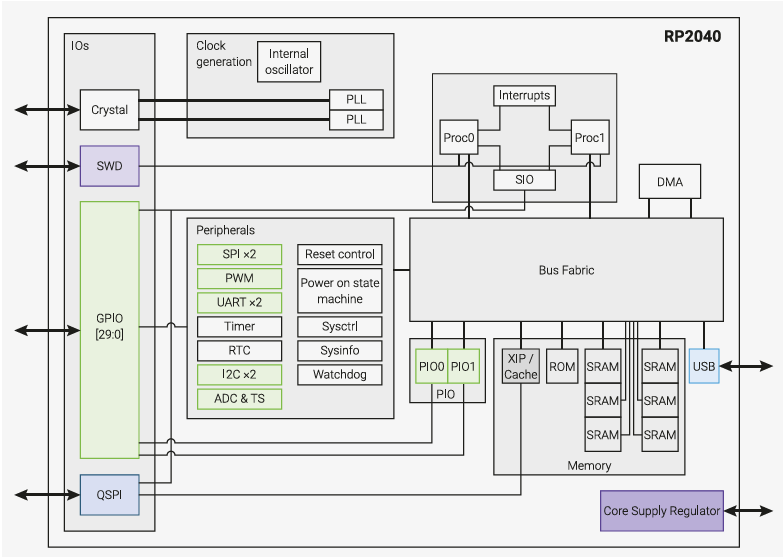
\includegraphics[width=0.6\textwidth]{rp2040_block_diagram.png}
        \caption{RP2040}
        \label{fig:RP2040}
    \end{figure}

    \item Przetwornika analogowo-cyfrowego 
    \begin{figure}[!ht]
        \centering
        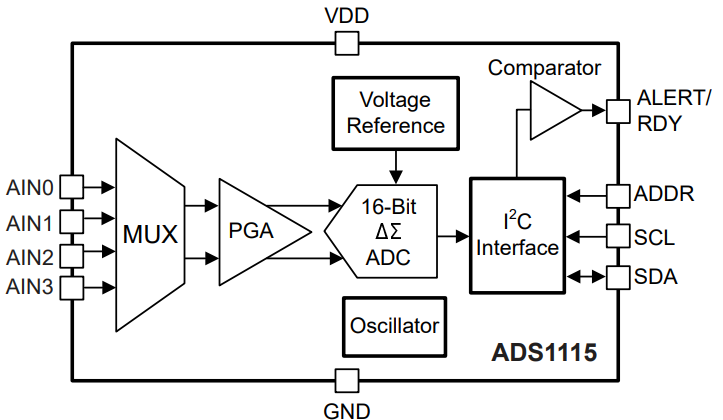
\includegraphics[width=0.6\textwidth]{ADC_block_diagram.png}
        \caption{ADS1115}
        \label{fig:ADS1115}
    \end{figure}

Schemat blokowy analizatora przedstawiono poniżej.
\begin{figure}[!ht]
    \centering
    \begin{circuitikz}
        \draw
            (0, 0) node[draw, minimum width = 6cm, minimum height = 3cm, align=center](PICO){\LARGE{Raspberry PI}\\\ \\\large{PICO W}}
            (3, -5)node[draw, minimum width = 12cm, minimum height = 3cm, align=center](PINS){\LARGE{Pin header}}

            (0, 4) node[draw, minimum width = 2cm, minimum height = 2cm](LDO){\LARGE{LDO}}
            % (5, 2) node[draw, minimum width = 2cm, minimum height = 2cm](V_REF){\LARGE{$\text{V}_{\text{ref}}$}}
            (6.5, 4) node[draw, minimum width = 2cm, minimum height = 2cm](ADC){\LARGE{ADC}}
            (5, 0) node[draw, minimum width = 2cm, minimum height = 2cm](AAF_PICO){\LARGE{AAF}}
            (8, 0) node[draw, minimum width = 2cm, minimum height = 2cm](AAF_ADC){\LARGE{AAF}}


            (PICO.west) to[short, -o] ++(-2, 0) node[above]{\large{USB}}
            (PICO.south) to[tmultiwire, l2=digital and logic, a=16] ++(0, -2)
            (LDO.south) to[short, a=$5V$] (PICO.north)

            (PICO.east) to[bmultiwire, l = 2] (AAF_PICO.west)
            (LDO) to[short, l=$3.3V$] (ADC) -| (8, 4) to[bmultiwire, l=2] (AAF_ADC.north)
            (ADC.south) --++ (0, -0.75) to[bmultiwire, a=$I^2C$] ++ (-5, 0) -- ++(0, -0.75)

            (AAF_PICO.south) to[bmultiwire, l=2] ++ (0, -2.5) 
            (AAF_ADC.south)  to[bmultiwire, l=2] ++ (0, -2.5)
        ;
    \end{circuitikz}
    \caption{Schemat blokowy analizatora stanów logicznych}
    \label{figure:block_diagram}
\end{figure}
\end{enumerate}



\useNormalLandscape{}
\section{Schemat ideowy analizatora}
    \begin{figure}[!ht]
        \centering
        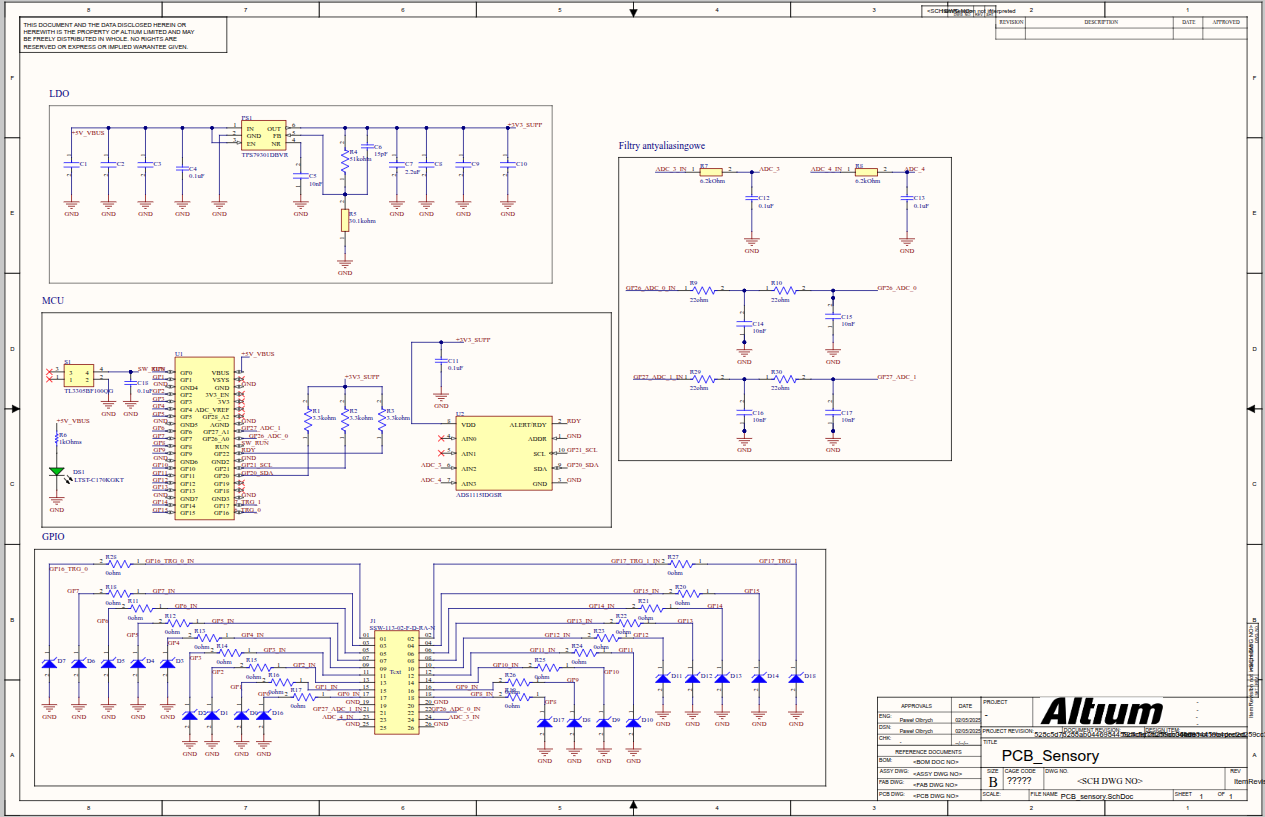
\includegraphics[width = 0.9\textwidth]{schematic.png}
        \caption{Schemat ideowy analizatora stanów logicznych}
    \end{figure}
\usePortrait{}

    Płytka PCB analizatora stanów logicznych o wymiarach 74.3mm x 59mm została zaprojektowana w oprogramowaniu Altium.
    Do poprowadzenia sygnałów miedzy blokami funkcyjnymi wykorzystano ścieżki na warstwie 1 i 4 o szerokości 10mil (0.254mm)
    oraz przelotki o wymiarach 0.3mm/0.6mm (otwór/średnica padu). Z uwagi na zastosowany stackup warstwa 2 i 3 pełnią funkcję
    ciągłej masy skracając drogę powrotu prądu sygnałowego (return path), co redukuje szumy i emisję EMI.
    W celu zapewnienia jednoczesnego próbkowania sygnałów wejściowych w analizatorze stanów logicznych, zachowano mniejwięcej 
    jednakowe długości ścieżek sygnałowych prowadzących do wejść mikrokontrolera. Różnice długości prowadzą do zmian w czasie propagacji
    sygnału, co może powodować błędnę rozpoznanie stanów logicznych lub zakłócenia synchronizacji danych. Zastosowano również
    przelotki typu \textit{via stitching} poprawiające ciągłość potencjału masy. Widok plików gerber warsty 1 oraz 4 przedstawiono
    na rysunku 4.3 i 4.4.
    

% \subsection{Stackup}
\paragraph{Stackup}
    Na rysunku \ref{fig:stackup}, przedstawiono wybrany stackup PCB proponowany przez firmę JLC PCB do projektów 4-o warstwowych.
    \begin{figure}[!ht]
        \centering
        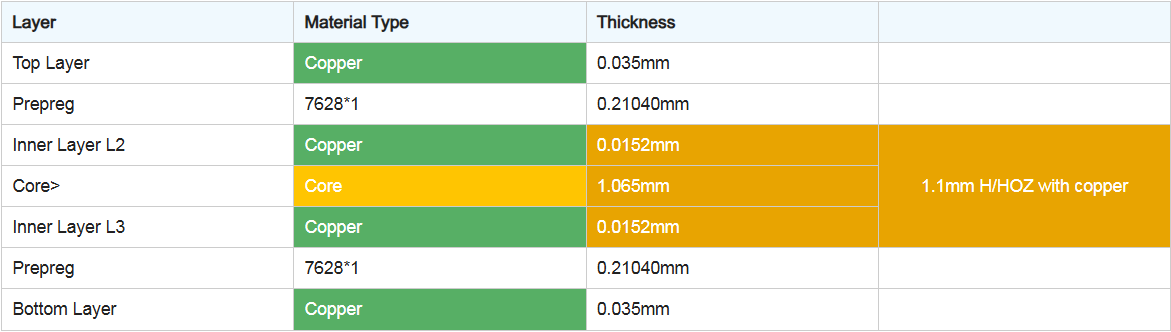
\includegraphics[width = 0.8\textwidth]{stackup.png}
        \caption{Stackup zalecany przez firmę JLC PCB}
        \label{fig:stackup}
    \end{figure}

     \begin{figure}[!ht]
        \centering
        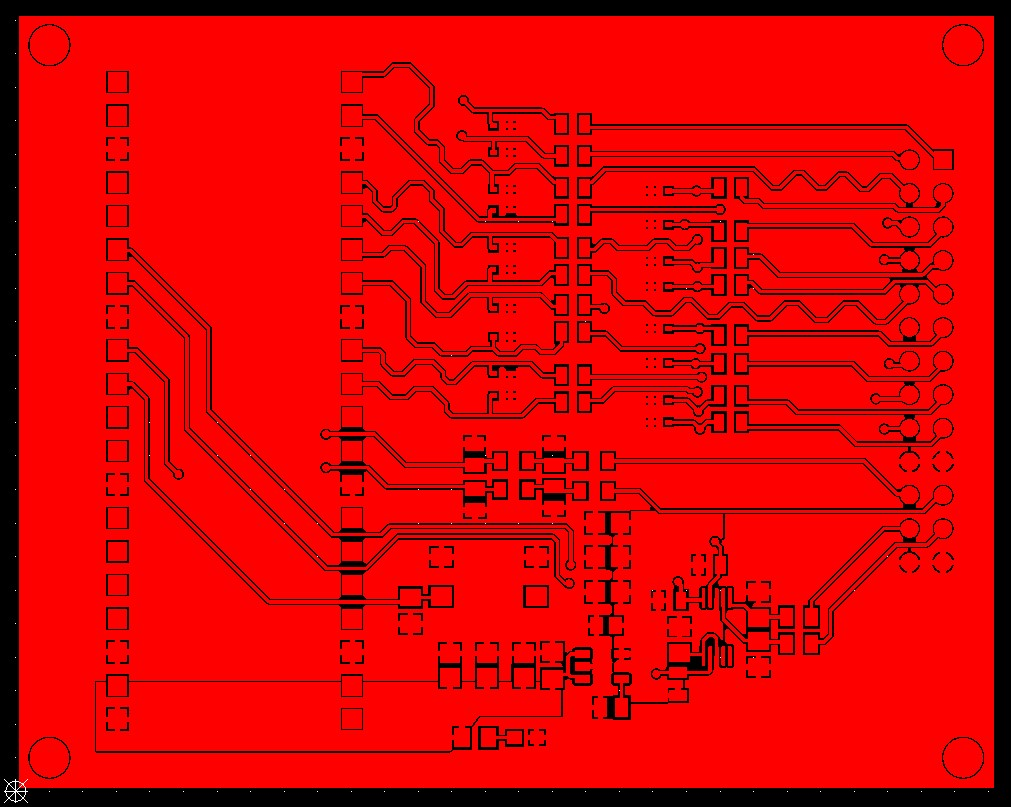
\includegraphics[width = 0.8\textwidth]{gerber_top.jpg}
        \caption{Widok pliku gerber warstwy 1 }
        \label{fig:gerber_top}
    \end{figure}

    \begin{figure}[!ht]
        \centering
        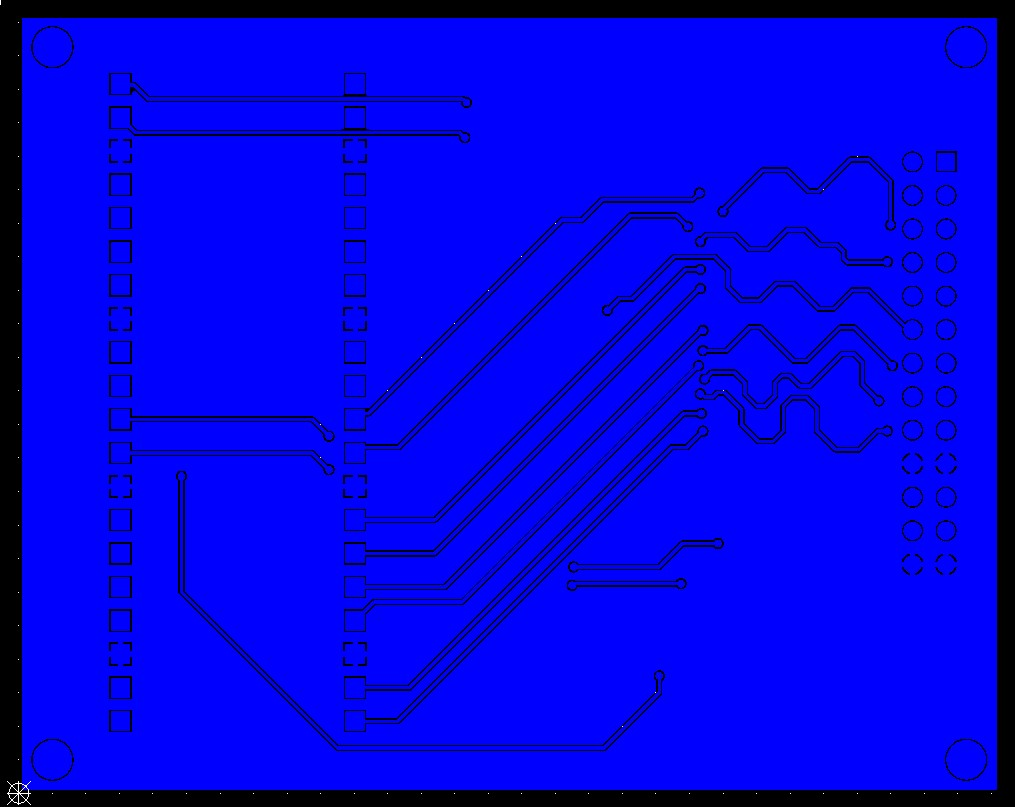
\includegraphics[width = 0.8\textwidth]{gerber_bottom.jpg}
        \caption{Widok pliku gerber warstwy 4 }
        \label{fig:gerber_bottom}
    \end{figure}
 

\subsection{Symulacje filtrów wejściowych}
Poniżej przedstawiono charakterystyki filtrów wejściowych sekcji analogowej.
\begin{figure}[!ht]
    \centering
    \begin{tikzpicture}
        \begin{axis}[
            width = 0.45\textwidth,
            grid = both,
            % axis lines= middle,
            % axis line style={->},
            xmin = 100, xmax = 10e3,
            xmode=log,
            title= Filtr ADS1115,
            ylabel = wzmocnienie ${[dB]}$,
            xlabel = częstotliwość ${[log(Hz)]}$
        ]
            \addplot table [x = freq, y =voltage, col sep = comma]{Measure/filter_ADS1115.csv};
            % \addplot table [x = duty, y = speedL, col sep = comma]{Measure/speed.csv};
        \end{axis}
    \end{tikzpicture}
    \begin{tikzpicture}
        \begin{axis}[
            width = 0.45\textwidth,
            grid = both,
            % axis lines= middle,
            % axis line style={->},
            xmin = 1e4, xmax = 3e6,
            xmode=log,
            title= Filtr PICO,
            ylabel = wzmocnienie ${[dB]}$,
            xlabel = częstotliwość ${[log(Hz)]}$
        ]
            \addplot table [x = freq, y =voltage, col sep = comma]{Measure/filter_PICO.csv};
            % \addplot table [x = duty, y = speedL, col sep = comma]{Measure/speed.csv};
        \end{axis}
    \end{tikzpicture}
    \caption{Wykresy tłumienia filtrów wejściowych}
\end{figure}